\chapter{搜索}

\section{人工智能}

\subsection{人工智能(Artificial Intelligence)}

我们称自己为智人,几千年来,我们一直试图了解我们是如何思考和行动的。\\

AI企图了解智能的实质,并生产出一种新的能以人类智能相似的方式做出反应的智能机器,该领域的研究包括机器人学、语言识别、图像识别、自然语言处理和专家系统等。\\

人类通过器官(眼、耳、鼻、口、皮肤)从外部环境进行感知,并做出一系列行为(说话、吃饭、移动、决策等)。\\

智能Agent通过传感器(麦克风、摄像头、陀螺仪、声呐等)从外部环境进行感知,从而进行规划、分类、预测等行为。\\

一个理性的Agent(Rational Agent)需要能进行理性的思考和行为,即在现有环境下,做出利益最大化的行为。\\

\subsection{AI的演变}

\subsubsection{基于逻辑的AI(Logic-Based AI)}

最初的人工智能是基于逻辑学的,数理逻辑的思想和方法一直在知识表示中发挥着重要作用。基于逻辑的AI的领域包括常识推理、溯因推理、归纳推理、计算逻辑、概率、规划、决策等。\\

建立在命题逻辑和谓词逻辑上的AI在九十年代前进入了寒冬,直到大量统计学方法引入之后才有了现在大热的机器学习。\\

\subsubsection{专家系统(Expert System)}

专家系统是一个智能计算机程序,其内部含有大量的某个领域专家水平的知识与经验,它根据系统中的知识与经验,进行推理和判断,模拟人类专家的决策过程,以便解决那些需要人类专家处理的复杂问题。\\

例如医疗诊断系统,它依靠病人的具体病况作为条件来分析,系统可根据病人的病情描述,在已有的知识与经验中,匹配最有可能的病症和治疗方案。\\

虽然专家系统看起来已经发展了很久,但是它并没有那么可靠。例如在实际的看病过程中,往往医生在除了问询之外,还有自己做推断的部分,目前的专家系统还没有办法做到对病人的病况了解的足够清晰。\\

其次专家系统的一大问题就是其潜在的风险性,包括无人驾驶汽车也有类似的问题。在发生问题之后,谁来背负责任呢?比如某患者采用了一个医疗专家系统,然后听从专家系统的指示,可结果病情却越来越重。\\

\subsubsection{机器学习(Machine Learning)}

机器学习是一门多领域交叉的学科,涉及概率论、统计学、逼近论、凸分析、算法复杂度理论等多门学科,专门研究计算机怎样模拟或实现人类的学习行为,以获取新的知识或技能,重新组织已有的知识结构使之不断改善自身的性能。\\

例如在自动驾驶中需要通过机器视觉不断看到周围的物体,然后通过机器学习来辨识出这些物体是什么(人、车、交通灯等)。学会辨识图片的过程需要输入大量的车辆的图片给机器学习,最后它就会知道这些图片代表的是车。

\begin{figure}[H]
    \centering
    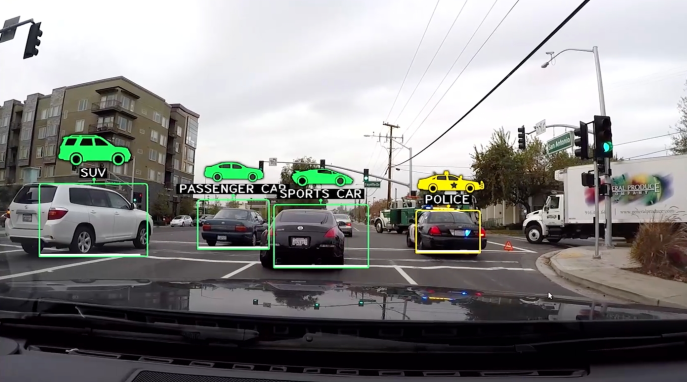
\includegraphics{img/C1/1-1/1.png}
    \caption{自动驾驶}
\end{figure}

机器学习最重要的是预测,比如通过大量的图片学会什么是车后,再来一张没有见过的车辆的图片,我们希望机器可以做出正确的判断。因此机器学习包含训练和预测两个部分,并且要保证一定的正确率。\\

\subsubsection{深度学习(Deep Learning)}

深度学习是一种深层次的学习,以教儿童认字为例,按照字从简单到复杂的顺序,让儿童反复看每个字的各种写法,并自己临摹。看得多了,自然就记住了。下次再见到同一个字,就很容易能认出来。认字时,一定是儿童的大脑在接受许多遍相似图像的刺激后,为每个字总结出了某种规律性的东西,下次大脑再看到符合这种规律的图案,就知道是什么字了。\\

计算机在识别时,也要先把每一个图案反复看很多很多遍,然后在总结出一个规律,以后计算机再看到类似的图案,只要符合之前总结的规律,计算机就能知道这是什么图案。用专业的术语来说,计算机用来学习的、反复看的图片叫训练数据集。

\begin{figure}[H]
    \centering
    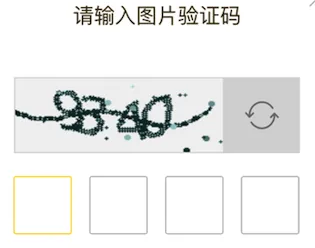
\includegraphics{img/C1/1-1/2.png}
    \caption{验证码}
\end{figure}

深度学习与机器学习的主要区别是在于性能。当数据量很少的时候,深度学习的性能并不好,因为深度学习算法需要大量数据才能很好理解其中蕴含的模式。因此深度学习算法严重依赖高端机,而传统的机器学习算法在低端机上就能运行。深度学习需要GPU(Graphics Processing Unit)进行大量的矩阵乘法运算。

\newpage

\section{状态空间}

\subsection{智能Agent}

智能Agent的设计取决于一系列因素:

\begin{itemize}
    \item 环境:静态(static)、动态(dynamic)
    \item 表示方案(representation scheme):状态(state)、特征(feature)、关系(relation)
    \item 可观察性(observability):完全可观察、部分可观察
    \item 参数类型:离散(discrete)、连续(continuous)
    \item 不确定性(uncertainty):确定性(deterministic)、随机性(stochastic)
    \item 学习:知识是给定的(已知的),知识是学来的(未知的)
    \item Agent数量:单Agent、多Agent
\end{itemize}

\vspace{0.5cm}

\subsection{状态空间(State Space)}

假设有两个有灰尘的房间A和B,吸尘器一开始位于房间A,吸尘器只能进行左移、右移和吸尘三个操作,最终的目标是将两个房间内的灰尘清扫完毕。\\

因此根据房间有无灰尘和吸尘器的位置,一共存在8种状态。

\begin{figure}[H]
    \centering
    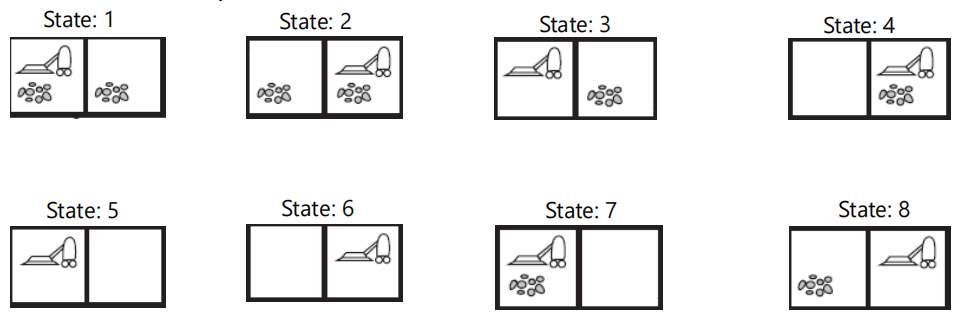
\includegraphics[scale=0.7]{img/C1/1-2/1.png}
\end{figure}

\begin{table}[H]
    \centering
    \setlength{\tabcolsep}{5mm}{
        \begin{tabular}{|c|c|c|c|}
            \hline
            \textbf{状态} & \textbf{房间A} & \textbf{房间B} & \textbf{吸尘器位置} \\
            \hline
            1             & 脏             & 脏             & A                   \\
            \hline
            2             & 脏             & 脏             & B                   \\
            \hline
            3             & 干净           & 脏             & A                   \\
            \hline
            4             & 干净           & 脏             & B                   \\
            \hline
            5             & 干净           & 干净           & A                   \\
            \hline
            6             & 干净           & 干净           & B                   \\
            \hline
            7             & 脏             & 干净           & A                   \\
            \hline
            8             & 脏             & 干净           & B                   \\
            \hline
        \end{tabular}
    }
\end{table}

假设以状态6作为目标状态(goal state),可以得到状态空间图:

\begin{figure}[H]
    \centering
    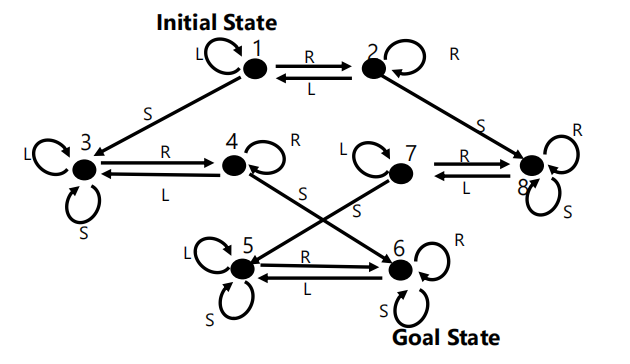
\includegraphics{img/C1/1-2/2.png}
\end{figure}

提取问题中的特征:

\begin{itemize}
    \item $ status = \{clean, dirty\} $
    \item $ location = \{A, B\} $
    \item $ actions = \{suck, left, right\} $
\end{itemize}

吸尘器的处理过程可以表示为:

\begin{algorithm}[H]
    \caption{VacuumCleaner}
    \begin{algorithmic}[1]
        \Procedure{VacuumCleaner}{status, location}
        \If {status = dirty}
        \State \Return suck
        \EndIf

        \If {location = A and status = clean}
        \State \Return right
        \EndIf

        \If {location = B and status = clean}
        \State \Return left
        \EndIf
        \EndProcedure
    \end{algorithmic}
\end{algorithm}

\vspace{0.5cm}

\subsection{性能评估(Performance Measure)}

算法的性能评估包含以下几个方面:

\begin{itemize}
    \item 完备性(completeness)
          \begin{itemize}
              \item 完备(Complete):算法可以到达目标状态
              \item 不完备(incomplete):算法无法到达目标状态
          \end{itemize}
    \item 正确性
    \item 最优性(optimality):算法以最优解(最小代价)找到到达目标状态的路径
    \item 时间复杂度(time complexity):求解所需的时间
    \item 空间复杂度(space complexity):求解所需的存储空间
\end{itemize}

\newpage

\section{盲目搜索/无信息搜索}

\subsection{盲目搜索/无信息搜索(Uninformed Search)}

当需要采取的正确行动不是显而易见时,Agent就需要提前规划,考虑能够通往目标状态的一系列行动,Agent所进行的计算过程被称为搜索。\\

对于一个问题,首先需要确定它的初始状态(initial state)和目标状态,其次需要对问题进行建模(modeling)。一个问题的建模包括6个部分:

\begin{enumerate}
    \item 状态集合
    \item 初始状态
    \item 行为集合$ Actions(s) $:在状态$ s $时所有合法的行为集合
    \item 状态转移$ Result(s, a) $:返回在状态$ s $时执行行为$ a $后的状态
    \item 目标状态:使用$ IsGoal(s) $来判断状态$ s $是否为目标状态
    \item 行为代价函数(Action Cost Function):在某个状态执行某个行为所需的代价,使用$ ActionCost(s, a, s') $表示在状态$ s $执行行为$ a $到达状态$ s' $所需的代价
\end{enumerate}

在八数码(8-puzzle)问题中,在一个3*3的方格中,有数字1~8和一个空白,最终需要将数字依次排列,使空白位于最后的位置。\\

八数码问题一共存在$ 9! = 362880 $种状态,其中初始状态为任意一种摆放布局,目标状态为依次排列的布局。

\begin{figure}[H]
    \centering
    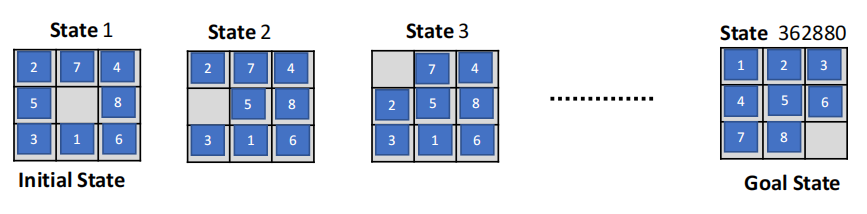
\includegraphics[scale=0.8]{img/C1/1-3/1.png}
\end{figure}

行为包括可以将空白进行上移(U)、下移(D)、左移(L)、右移(R),每次移动的代价可以认为都为1,例如对初始状态中的空白进行左移,其状态转移可表示为$ s_2 = Result(s_1, L) $。\\

在罗马尼亚地图(Romania map)中,例如初始位置位于Arad,最终想要到达Bucharest。问题的状态为所有的城市,每次行动的代价为城市见的距离。

\begin{figure}[H]
    \centering
    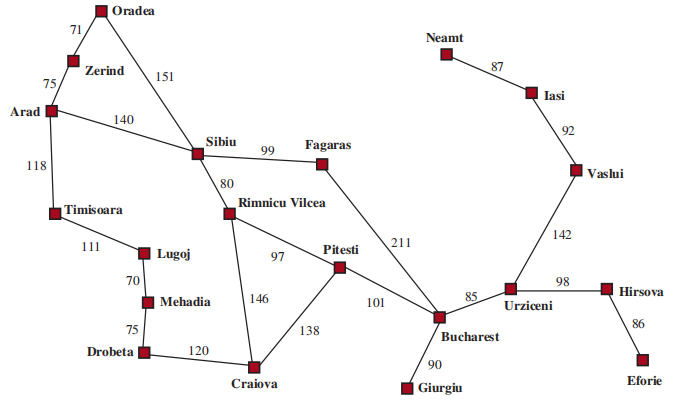
\includegraphics{img/C1/1-3/2.png}
    \caption{罗马尼亚地图}
\end{figure}

\vspace{0.5cm}

\subsection{搜索树(Search Tree)}

搜索树中的每个结点对应于状态空间中的一个状态,边对应着行为,根结点对应于初始状态。\\

搜索树从根结点开始,每次选择一个结点进行扩展(expand),扩展的过程是递归的,直到搜索到目标状态。\\

搜索树中的每个结点由4部分组成:

\begin{enumerate}
    \item node.State:状态信息(如Sibiu)
    \item node.Parent:父结点(如Arad),用于回溯
    \item node.Action:从父结点到当前结点的行为(如ToSibiu)
    \item node.PathCost:从根结点到当前结点的代价,用于查找最优解
\end{enumerate}

\begin{figure}[H]
    \centering
    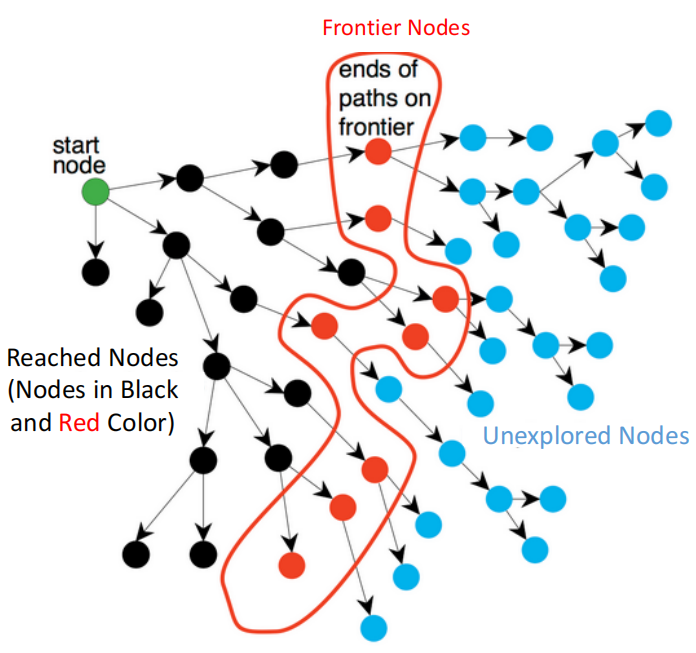
\includegraphics[scale=0.8]{img/C1/1-3/3.png}
    \caption{搜索树}
\end{figure}

\begin{algorithm}[H]
    \caption{Expand a node}
    \begin{algorithmic}[1]
        \Procedure{Expand}{problem, node} yield nodes
        \State s = node.State

        \For {action in problem.Actions(s)}
        \State s' = problem.Result(s, action)
        \State cost = node.PathCost + problem.ActionCost(s, action, s')
        \State yield Node(State=s', Parent=node, Action=action, PathCost=cost)
        \EndFor
        \EndProcedure
    \end{algorithmic}
\end{algorithm}

\begin{figure}[H]
    \centering
    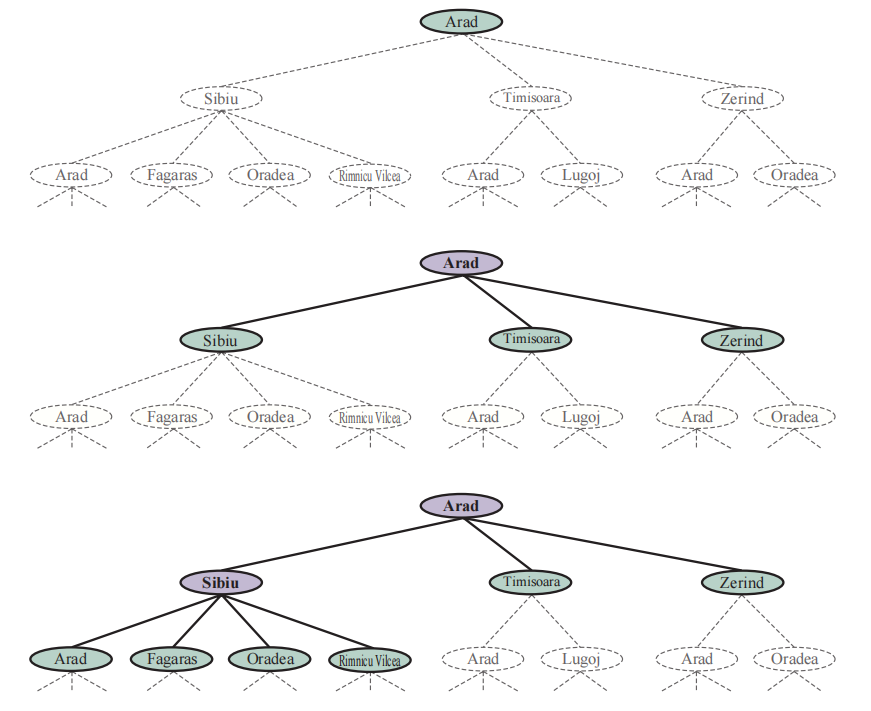
\includegraphics[scale=0.8]{img/C1/1-3/4.png}
\end{figure}

所有已经到达的结点(reached node)都保存在一个哈希表中,以便于避免重复搜索。\\

而所有前沿结点(frontier node)根据不同的搜索策略,可以使用栈、队列或优先队列保存,从而觉得后续需要扩展的结点。

\newpage

\section{盲目搜索策略}

\subsection{广度优先搜索(BFS, Breadth-First Search)}

\begin{figure}[H]
    \centering
    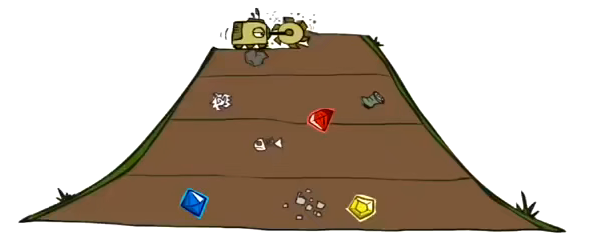
\includegraphics{img/C1/1-4/1.png}
    \caption{BFS}
\end{figure}

BFS首先把从源点相邻的顶点遍历,然后再遍历稍微远一点的顶点,再去遍历更远一点的顶点。\\

\begin{figure}[H]
    \centering
    \begin{tikzpicture}[
            level distance=1.5cm,
            level 1/.style={sibling distance=4cm},
            level 2/.style={sibling distance=2cm},
            level 3/.style={sibling distance=1cm}
        ]
        \node[circle,draw] {1}
        child {
                node[circle,draw] {2}
                child {
                        node[circle,draw] {4}
                        child {node[circle,draw] {8}}
                        child {node[circle,draw] {9}}
                    }
                child {
                        node[circle,draw] {5}
                        child {node[circle,draw] {10}}
                        child {node[circle,draw] {11}}
                    }
            }
        child {
                node[circle,draw] {3}
                child {
                        node[circle,draw] {6}
                        child {node[circle,draw] {12}}
                        child {node[circle,draw] {13}}
                    }
                child {
                        node[circle,draw] {7}
                        child {node[circle,draw] {14}}
                        child {node[circle,draw] {15}}
                    }
            };
    \end{tikzpicture}
\end{figure}

\begin{algorithm}[H]
    \caption{BFS}
    \begin{algorithmic}[1]
        \Procedure{BFS}{problem} returns a solution node or failure
        \State node = Node(problem.Initial)

        \If {problem.IsGoal(node.State)}
        \State \Return node
        \EndIf
        \\
        \State frontier = Queue(node)
        \State reached = {problem.Initial}
        \\
        \While {not IsEmpty(frontier)}
        \State node = frontier.dequeue()
        \For {child in Expand(problem, node)}
        \State s = child.State
        \If {problem.IsGoal(s)}
        \State reutnr child
        \EndIf
        \If {s is not in reached}
        \State reached.add(s)
        \State frontier.enqueue(child)
        \EndIf
        \EndFor
        \EndWhile
        \\
        \State \Return failure
        \EndProcedure
    \end{algorithmic}
\end{algorithm}

\begin{itemize}
    \item 时间复杂度:$ O(b^d) $
    \item 空间复杂度:$ O(b^d) $(最多需要保存最后一层结点的数量)
    \item 完备性:YES(当$ d $有穷)
    \item 最优性:YES(总能找到最浅的目标结点)
\end{itemize}

\vspace{0.5cm}

\subsection{深度优先搜索(DFS, Depth-First Search)}

\begin{figure}[H]
    \centering
    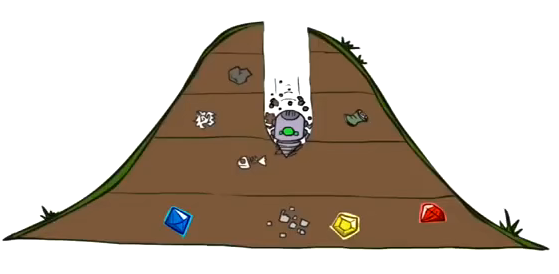
\includegraphics{img/C1/1-4/2.png}
    \caption{DFS}
\end{figure}

深度优先搜索是一种一头扎到底的遍历方法,选择一条路,尽可能不断地深入,遇到死路就回退,回退过程中如果遇到没探索的支路,就进入该支路继续深入。\\

\begin{figure}[H]
    \centering
    \begin{tikzpicture}
        \begin{scope}[every node/.style={circle,thick,draw}]
            \node (0) at (2.5,4) {0};
            \node (1) at (5,3) {1};
            \node (2) at (2.5,2) {2};
            \node (3) at (1,0) {3};
            \node (4) at (3,0) {4};
            \node (5) at (5,1) {5};
            \node (6) at (6,-1) {6};
            \node (7) at (0,3) {7};
        \end{scope}

        \begin{scope}[>={Stealth[black]},
            every node/.style={},
            every edge/.style={draw=black,very thick}]
            \path [-] (0) edge node {} (1);
            \path [-] (0) edge node {} (2);
            \path [-] (0) edge node {} (7);
            \path [-] (1) edge node {} (4);
            \path [-] (1) edge node {} (5);
            \path [-] (2) edge node {} (4);
            \path [-] (3) edge node {} (4);
            \path [-] (5) edge node {} (6);
        \end{scope}
    \end{tikzpicture}
\end{figure}

\begin{algorithm}[H]
    \caption{DFS}
    \begin{algorithmic}[1]
        \Procedure{DFS}{problem} returns a solution node or failure
        \State node = Node(problem.Initial)

        \If {problem.IsGoal(node.State)}
        \State \Return node
        \EndIf
        \\
        \State frontier = Stack(node)
        \\
        \While {not IsEmpty(frontier)}
        \State node = frontier.pop()
        \If {problem.IsGoal(s)}
        \State reutnr node
        \EndIf
        \\
        \If {not IsCycle(node)}
        \For {child in Expand(problem, node)}
        \State frontier.push(child)
        \EndFor
        \EndIf
        \EndWhile
        \\
        \State \Return failure
        \EndProcedure
    \end{algorithmic}
\end{algorithm}

\begin{itemize}
    \item 时间复杂度:$ O(b^m) $(当$ m $有穷)
    \item 空间复杂度:$ O(bm) $(只需要保存一层的兄弟结点)
    \item 完备性:NO(当$ m $无穷)
    \item 最优性:NO(只能找到最左解)
\end{itemize}

\vspace{0.5cm}

\subsection{深度限制搜索(DLS, Depth-Limit Search)}

DLS是DFS的变体,它限制了访问的深度。因为当树的子树过深时,进行DFS会在该子树上消耗太多的时间,所以在DLS中,若该结点的深度大于限制深度$ l $,那就不再继续遍历其子树了。\\

\begin{algorithm}[H]
    \caption{DLS}
    \begin{algorithmic}[1]
        \Procedure{DLS}{problem, l} returns a solution node or failure or cutoff
        \State frontier = Stack(problem.Initial)
        \State result = failure
        \\
        \While {not IsEmpty(frontier)}
        \State node = frontier.pop()
        \If {Depth(node) > l}
        \State result = cutoff
        \ElsIf {not IsCycle(node)}
        \For {child in Expand(problem, node)}
        \State frontier.push(child)
        \EndFor
        \EndIf
        \EndWhile
        \\
        \State \Return result
        \EndProcedure
    \end{algorithmic}
\end{algorithm}

\begin{itemize}
    \item 时间复杂度:$ O(b^l) $
    \item 空间复杂度:$ O(bl) $
    \item 完备性:NO
    \item 最优性:NO
\end{itemize}

\vspace{0.5cm}

\subsection{迭代加深搜索(IDS, Iterative Deepening Search)}

IDS是DLS的升级版本,即首先允许深度优先搜索$ k $层搜索树,若没有发现可行解,再将$ k + 1 $后重复以上步骤搜索。\\

IDS将DFS的空间优势和BFS的时间优势结合起来,是一种比较好的搜索算法。\\

\begin{algorithm}[H]
    \caption{IDS}
    \begin{algorithmic}[1]
        \Procedure{IDS}{problem} returns a solution node or failure
        \For {depth = 0 to $ \infty $}
        \State result = DLS(problem, depth)
        \If {result != cutoff}
        \State \Return result
        \EndIf
        \EndFor
        \EndProcedure
    \end{algorithmic}
\end{algorithm}

\begin{itemize}
    \item 时间复杂度:$ O(b^d) $
    \item 空间复杂度:$ O(bd) $
    \item 完备性:YES
    \item 最优性:YES
\end{itemize}

\vspace{0.5cm}

IDS很明显存在重复的搜索,在迭代至第$ k $层时,会重复搜索前$ k - 1 $层的所有结点。虽然这的确浪费了一些时间,但是它并没有那么不堪。\\

假设分别计算使用BFS和IDS所生成的结点数量:

\vspace{-1cm}

\begin{align*}
    N(BFS) & = 1 + b^1 + b^2 + \cdots + b^d                    \\
    N(IDS) & = (d)b +  (d - 1)b^2 + (d-2)b^3 + \cdots + (1)b^d
\end{align*}

假设$ b = 10 $,$ d = 5 $时,$ N(BFS) = 111110 $,$ N(IDS) = 123450 $。可以计算得出IDS只比BFS多生成了11\%的结点。

\vspace{-1cm}

\begin{align*}
    {{N(IDS) - N(BFS)} \over {N(BFS)}} = 11\%
\end{align*}

因此,IDS只多生成了少量的结点,而节省了大量的空间。\\

\subsection{一致代价搜索(UCS, Uninformed-Cost Search)}

由于不同的行为具有不同的代价,每次选择一个从根结点到当前结点成本最低的路径是一个很好的选择。这被理论计算机科学界称为Dijkstra算法,被AI领域称为统一成本搜索UCS。BFS可以看作是根据树的深度一层一层扩展的,而UCS则是根据树的代价扩展的。\\

在罗马尼亚的部分地图中,问题是从Sibiu到达Bucharest。\\

\begin{figure}[H]
    \centering
    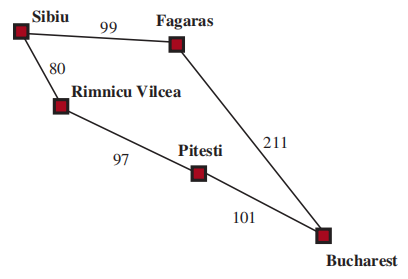
\includegraphics{img/C1/1-4/3.png}
\end{figure}

Sibiu的后继结点是Rimnicu Vilcea和Fagaras,路径成本分别为$ 80 $和$ 99 $。因此扩展代价最低的结点Rimnicu Vilcea,计算得出到Pitesti的路径代价为$ 80 + 97 = 177 $。\\

其次路径代价最低的是Fagaras,计算得出到Bucharest的路径代价为$ 99 + 211 = 310 $。此时,虽然Bucharest是目标状态,但是UCS算法并不会在生成结点时判断其是否为目标状态,而是在扩展结点的时候判断。\\

因此算法会继续选择Pitesti进行扩展,计算得出到Bucharest的路径代价为$ 80 + 97 + 101 = 278 $。这个具有更小的路径代价,因此它替换之前到达这里的路径,并被添加到前沿结点集合中。最终,它在被扩展时发现是目标状态。\\

\begin{algorithm}[H]
    \caption{UCS}
    \begin{algorithmic}[1]
        \Procedure{UCS}{problem} returns a solution node or failure
        \State \Return BestFirstSearch(problem, PathCost)
        \EndProcedure
        \\
        \Procedure{BestFirstSearch}{problem, PathCost}
        \State node = Node(problem.Initial)
        \State frontier = PriorityQueue(node)   \# ordered by PathCost
        \State reached = \{problem.Initial: node\}
        \\
        \While {not IsEmpty(frontier)}
        \State node = frontier.pop()
        \If {problem.IsGoal(node.State)}
        \State \Return node
        \EndIf
        \\
        \For {child in Expand(problem, node)}
        \State s = child.State
        \If {s is not in reached or child.PathCost < reached[s].PathCost}
        \State reached[s] = child
        \State frontier.push(child)
        \EndIf
        \EndFor
        \EndWhile
        \\
        \State \Return failure
        \EndProcedure
    \end{algorithmic}
\end{algorithm}

\begin{itemize}
    \item 时间复杂度:$ O(b^{1 + \lfloor C^* / \epsilon \rfloor}) $
    \item 空间复杂度:$ O(b^{1 + \lfloor C^* / \epsilon \rfloor}) $
    \item 完备性:YES
    \item 最优性:YES
\end{itemize}

\newpage